\documentclass[10pt,twocolumn]{article}
\usepackage[margin=1.7cm]{geometry}
\usepackage[T1]{fontenc}
\usepackage[utf8]{inputenc}
\usepackage{graphicx,booktabs,amsmath,microtype,hyperref}
\title{Automated Non-Contact Assessment of Bread Size and Shape\\
from RGB Images Using Computer Vision}
\author{AUTHOR\_NAME}
\date{}
\begin{document}
\maketitle
\begin{abstract}
We present a reproducible RGB computer-vision pipeline for bread dimension measurement. The
official Mendeley Data v1 archive was audited before modelling: 171 of 173 measurement rows were
uniquely usable and split by physical sample into train, validation and an untouched test set.
Otsu segmentation and contour morphology were compared with classical regressors and a frozen
MobileNetV3-Small baseline. Validation selected hist\_gradient\_boosting. On 26 test samples it achieved
MAE 2.10 for width and 2.40 for height, with $R^2$ 0.694 and 0.847.
Classical processing required 4.3 ms/image on CPU. The work supplies an auditable baseline
while retaining unit, calibration and external-validity limitations.
\end{abstract}
\textbf{Keywords:} computer vision; bread quality; non-destructive measurement; image
processing; machine learning; quality control.

\section{Introduction}
Manual bread inspection is intermittent and difficult to trace. Controlled RGB imaging offers a
low-cost alternative, but scale, pose and acquisition conditions can dominate accuracy. Prior
reviews describe extensive colour, texture and shape analysis while identifying limited
standardisation and reproducibility \cite{olakanmi2023review,martinezlara2026review}. We ask
whether an auditable morphology-based pipeline improves on one-dimensional pixel calibration.

\section{Materials and methods}
The CC BY 4.0 dataset by Mora \cite{mora2025bread_dataset} was downloaded from its versioned
record and kept outside Git. Its size CSV has 173 rows. A duplicated canonical image identifier
with conflicting targets caused two rows to be excluded, leaving 171 unique samples. CSV indices
without leading zeroes were linked to files through a strict view--batch--integer parser, never
through fuzzy matching. The dataset omits an explicit target unit; results therefore use a
nominal dataset unit (interpreted as mm) and preserve this as a limitation.

Images were converted to grayscale, smoothed, segmented with two-polarity Otsu thresholding
\cite{otsu1979threshold}, cleaned morphologically and reduced to the largest valid contour.
Features included bounding-box dimensions, area, perimeter, aspect ratio, circularity, solidity,
extent, equivalent diameter and ellipse descriptors. Physical sample IDs were divided
119/26/26
into train/validation/test with seed 42 and asserted to have zero overlap.

The archive audit examined 2211 readable images across size, colour and texture folders.
Only the width/height \texttt{E} view from the size folder entered this experiment. Derived
colour crops and the separate thickness \texttt{C} view were excluded from predictors,
preventing alternate views of the same physical item from crossing partitions.
Table~\ref{tab:data} summarises the auditable
sample flow; all exclusions remain in the generated manifest with an explicit reason.

\begin{table}[h]
\centering
\caption{Audited dataset and fixed experimental partition.}
\label{tab:data}
\begin{tabular}{lr}
\toprule Quantity & Count \\
\midrule Archive images & 2211 \\
Measurement CSV rows & 173 \\
Eligible physical samples & 171 \\
Train / validation / test & 119 / 26 / 26 \\
Segmentation failures & 0 \\
\bottomrule
\end{tabular}
\end{table}

Separate linear pixel calibrations were compared with linear, ridge, random-forest
\cite{breiman2001random} and histogram-gradient-boosting regressors. A frozen MobileNetV3-Small
\cite{howard2019mobilenetv3} head was selected by validation loss without test access. Classical
models were refit on train+validation after validation selection. Metrics were MAE, RMSE, MAPE,
$R^2$, bootstrap MAE intervals, paired Wilcoxon error tests and Bland--Altman agreement
\cite{bland1986agreement}.

All transformations were implemented as one command from a versioned YAML configuration. Random
seeds, package versions, the Git revision, a source-tree digest and hardware descriptors are
written to provenance. Test-set segmentation failure is a blocking error rather than a silently
dropped observation. Bootstrap intervals use the configured 2,000 resamples, and all paired
comparisons operate on identical physical sample IDs.

\begin{figure}[h]
\centering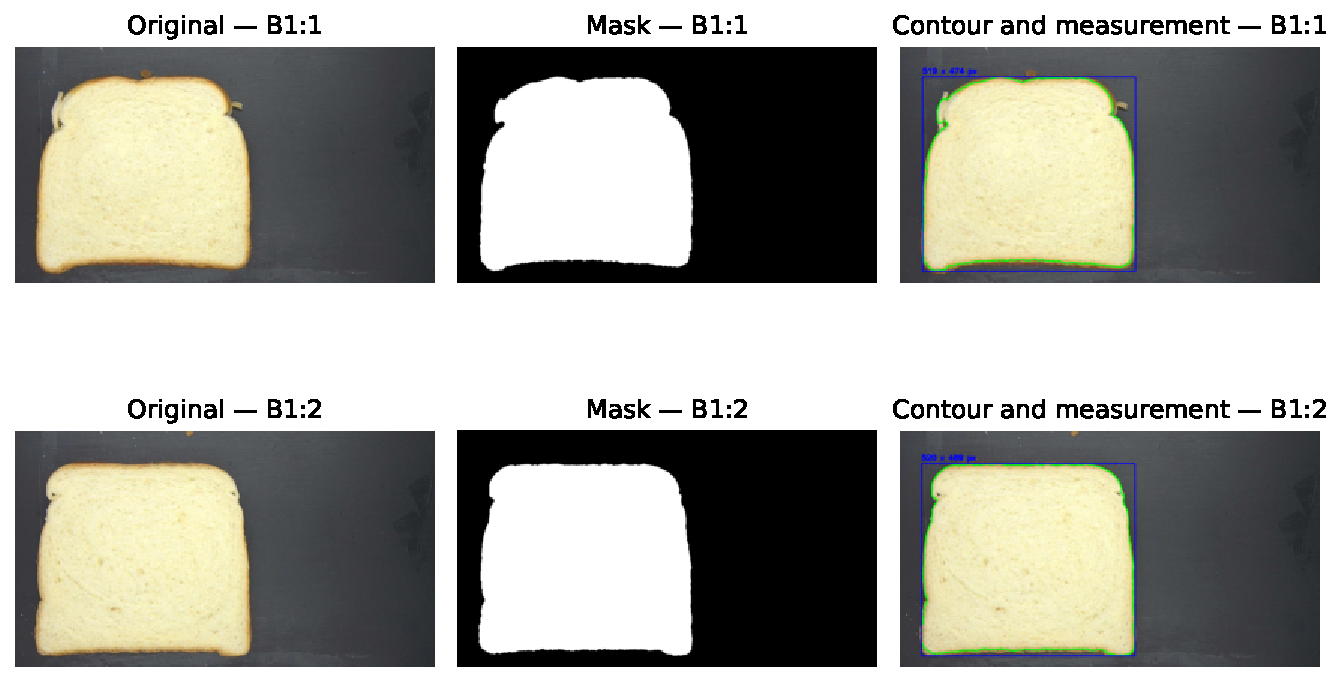
\includegraphics[width=\columnwidth]{figures/segmentation_examples.pdf}
\caption{Examples of source images, binary masks and retained contours.}
\end{figure}

\section{Results}
The validation-selected method was hist\_gradient\_boosting. Table~\ref{tab:results} reports final-test
performance. It improved width MAE over linear calibration from 4.55 to 2.10;
height MAE changed from 3.00 to 2.40. The CNN test MAEs were 2.83 and
4.52, so it did not displace the compact morphology model on this sample size.

\begin{table}[h]
\centering
\caption{Final-test performance in the nominal dataset unit.}
\label{tab:results}
\begin{tabular}{lrrr}
\toprule Target & MAE & RMSE & $R^2$ \\
\midrule Width & 2.10 & 3.12 & 0.694 \\
Height & 2.40 & 3.02 & 0.847 \\
\bottomrule
\end{tabular}
\end{table}

\begin{figure}[h]
\centering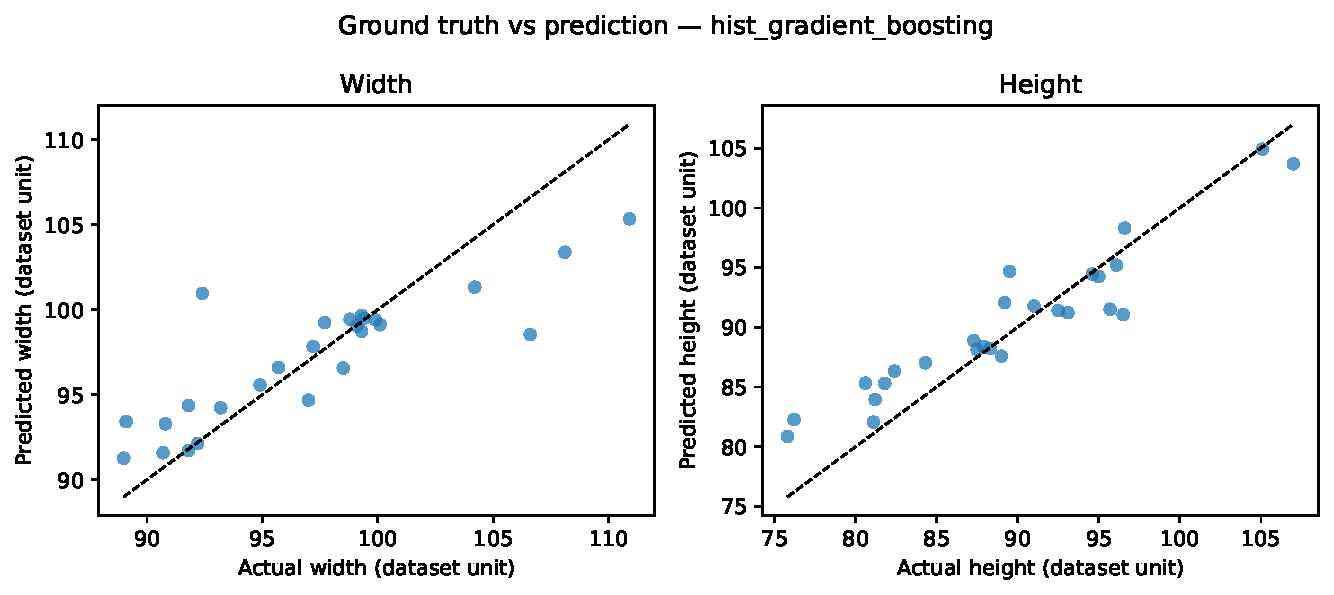
\includegraphics[width=\columnwidth]{figures/predicted_vs_actual.pdf}
\caption{Ground truth versus prediction for the validation-selected method.}
\end{figure}

All 171 eligible images segmented successfully. Classical segmentation and feature extraction
averaged 4.3 ms/image. The ablation, confidence intervals, per-sample predictions and
agreement limits are generated from the same run and retained in the repository.

The selected model's Bland--Altman width bias was close to zero, while the observed limits of
agreement remained wide enough to preclude interchangeability claims for precision metrology.
The paired improvement over the linear calibration was stronger for width than height. These
results support the narrower conclusion that morphology helps calibration under this controlled
setup; they do not establish a universal bread-quality score.

\begin{figure}[h]
\centering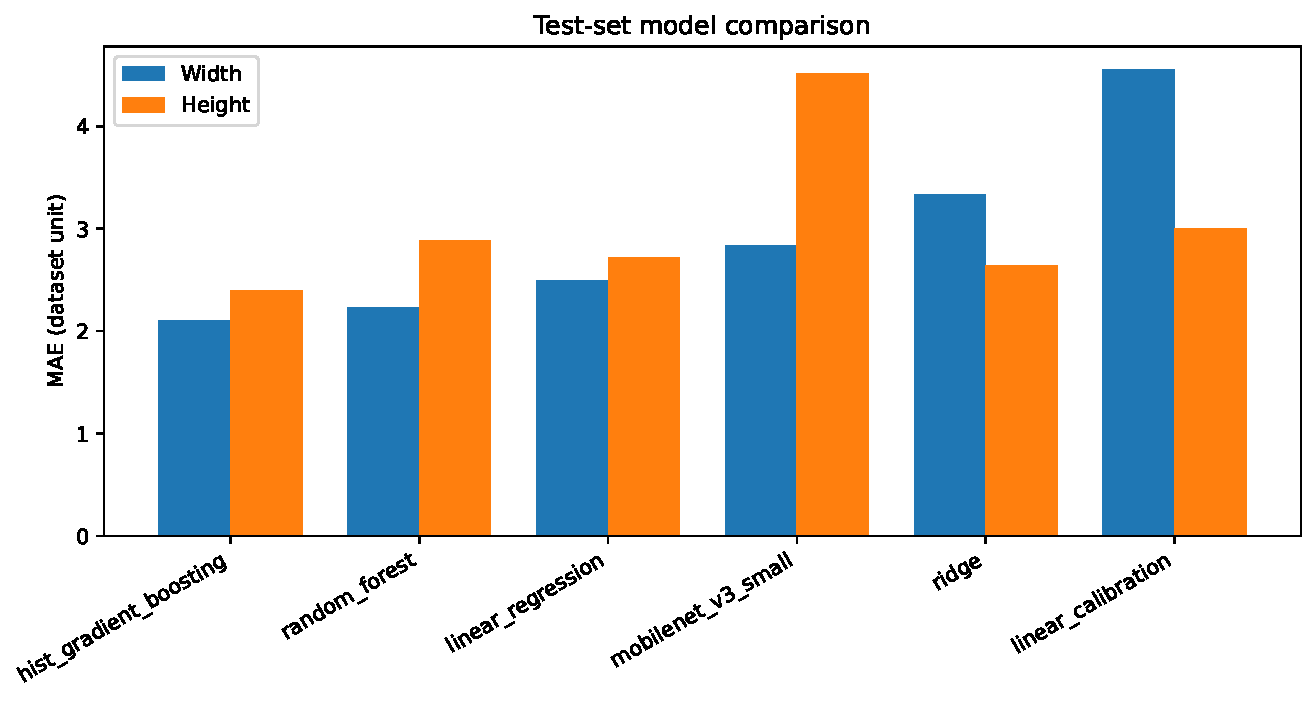
\includegraphics[width=\columnwidth]{figures/model_comparison.pdf}
\caption{Final-test MAE across the evaluated methods.}
\end{figure}

\section{Discussion and conclusion}
Morphology substantially improved width estimation over pixel-only calibration, while the height
gain was smaller. Irregular boundaries, pose and axis-aligned boxes remain error sources. The
small test set widens uncertainty, and no claim transfers across cameras or products without
external validation. A reference scale, prospective acquisition and instrument-uncertainty study
are necessary before deployment. Nevertheless, the project provides a fully traced baseline from
audit and grouped splitting through statistics, figures and reports.

The lightweight CNN underperformed the best classical regressor, which is plausible with only
119 training samples and a frozen generic backbone. This negative comparison is retained to
avoid selective reporting. Future work should evaluate rotated boxes or learned segmentation,
collect repeat instrument measurements, and test product- and camera-held-out cohorts. Deployment
should also monitor segmentation flags and acquisition drift rather than relying on a point
prediction alone.

\bibliographystyle{plain}
\bibliography{references}
\end{document}
